\documentclass{beamer}
\usepackage{gb4e}
\usepackage{tikz}
\usepackage{color}
\usepackage{array}
\usepackage{multirow}
\usepackage{booktabs}
\usepackage{hyperref}

\newcommand{\corpus}[1]{\textit{#1}}

%Information to be included in the title page:
\title{Family trees of languages}
\author{Jinyuan Wu}

\usetheme{Madrid}

\begin{document}

\frame{\titlepage}

\begin{frame}
\frametitle{Introduction}

We use a family tree to represent the relations of people in a family.

\begin{center}
    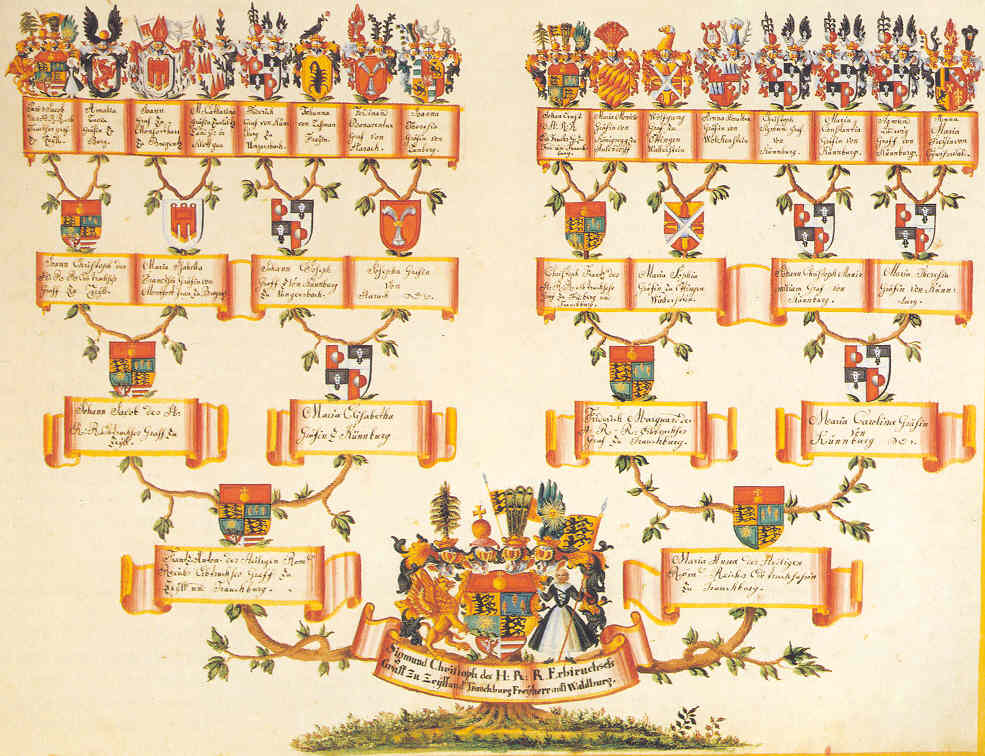
\includegraphics[width=0.6\textwidth]{photos/Waldburg-Ahnentafel.jpg}
\end{center} 

But what about languages?

\end{frame}

\begin{frame}
\frametitle{Languages evolve in their own ways}

\textbf{History of language $\neq$ history of people} 

\begin{itemize}
    \item Linguistic generic relation $\neq$ blood relation
\end{itemize}

``\textbf{Neogrammarian hypothesis}'':
changes can only arise from
\begin{itemize}
    \item Regular sound laws: \corpus{p} $>$ \corpus{f} 
    (in \emph{all} words when surrounded by certain other sounds)
    \item Borrowing: Arabic \corpus{ṣuffa} $>$ French \corpus{sofa} $>$ English \corpus{sofa} $>$ Mandarin Chinese \corpus{sh\={a}f\={a}} 
    \item Analogy (self-regularization): do you know once people said \corpus{baken} instead of \corpus{baked}?
\end{itemize}    

\end{frame}

\begin{frame}
\frametitle{The tree model of language evolution}

\begin{center}
    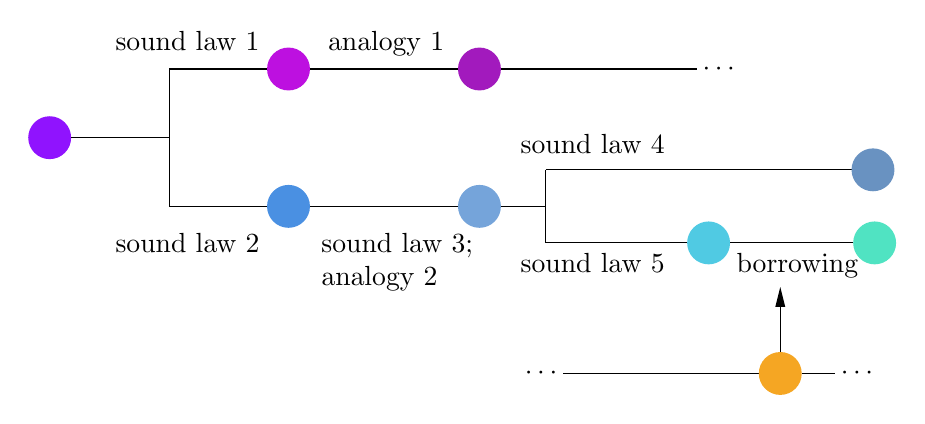
\begin{tikzpicture}[x=0.75pt,y=0.75pt,yscale=-0.8,xscale=0.8]
    %uncomment if require: \path (0,390); %set diagram left start at 0, and has height of 390
    
    %Shape: Circle [id:dp5224066501823912] 
    \draw  [draw opacity=0][fill={rgb, 255:red, 144; green, 19; blue, 254 }  ,fill opacity=1 ] (34,193.92) .. controls (34,186.78) and (39.78,181) .. (46.92,181) .. controls (54.05,181) and (59.83,186.78) .. (59.83,193.92) .. controls (59.83,201.05) and (54.05,206.83) .. (46.92,206.83) .. controls (39.78,206.83) and (34,201.05) .. (34,193.92) -- cycle ;
    %Straight Lines [id:da9727372947181603] 
    \draw    (59.83,193.92) -- (118.83,193.92) ;
    %Straight Lines [id:da6714571974898367] 
    \draw    (118.83,235.28) -- (118.83,152.55) ;
    %Straight Lines [id:da9057248721044227] 
    \draw    (118.83,152.55) -- (177.83,152.55) ;
    %Straight Lines [id:da8158449283595577] 
    \draw    (118.83,235.28) -- (177.83,235.28) ;
    %Shape: Circle [id:dp29865357440375595] 
    \draw  [draw opacity=0][fill={rgb, 255:red, 189; green, 16; blue, 224 }  ,fill opacity=1 ] (177.83,152.55) .. controls (177.83,145.42) and (183.62,139.64) .. (190.75,139.64) .. controls (197.88,139.64) and (203.67,145.42) .. (203.67,152.55) .. controls (203.67,159.69) and (197.88,165.47) .. (190.75,165.47) .. controls (183.62,165.47) and (177.83,159.69) .. (177.83,152.55) -- cycle ;
    %Shape: Circle [id:dp5543364890434692] 
    \draw  [draw opacity=0][fill={rgb, 255:red, 74; green, 144; blue, 226 }  ,fill opacity=1 ] (177.83,235.28) .. controls (177.83,228.15) and (183.62,222.36) .. (190.75,222.36) .. controls (197.88,222.36) and (203.67,228.15) .. (203.67,235.28) .. controls (203.67,242.41) and (197.88,248.2) .. (190.75,248.2) .. controls (183.62,248.2) and (177.83,242.41) .. (177.83,235.28) -- cycle ;
    %Straight Lines [id:da006468456223764685] 
    \draw    (203.67,152.55) -- (292.83,152.55) ;
    %Shape: Circle [id:dp4741527062200759] 
    \draw  [draw opacity=0][fill={rgb, 255:red, 162; green, 26; blue, 189 }  ,fill opacity=1 ] (292.83,152.55) .. controls (292.83,145.42) and (298.62,139.64) .. (305.75,139.64) .. controls (312.88,139.64) and (318.67,145.42) .. (318.67,152.55) .. controls (318.67,159.69) and (312.88,165.47) .. (305.75,165.47) .. controls (298.62,165.47) and (292.83,159.69) .. (292.83,152.55) -- cycle ;
    %Straight Lines [id:da5978409820875255] 
    \draw    (203.67,235.28) -- (292.83,235.28) ;
    %Shape: Circle [id:dp0131322414171402] 
    \draw  [draw opacity=0][fill={rgb, 255:red, 117; green, 164; blue, 218 }  ,fill opacity=1 ] (292.83,235.28) .. controls (292.83,228.15) and (298.62,222.36) .. (305.75,222.36) .. controls (312.88,222.36) and (318.67,228.15) .. (318.67,235.28) .. controls (318.67,242.41) and (312.88,248.2) .. (305.75,248.2) .. controls (298.62,248.2) and (292.83,242.41) .. (292.83,235.28) -- cycle ;
    %Straight Lines [id:da0536655628532241] 
    \draw    (318.67,235.28) -- (345.67,235.28) ;
    %Straight Lines [id:da3837604603337088] 
    \draw    (345.67,257.28) -- (345.67,213.28) ;
    %Straight Lines [id:da04939381997317582] 
    \draw    (345.67,213.28) -- (529.83,213.28) ;
    %Straight Lines [id:da9159881089317645] 
    \draw    (345.67,257.28) -- (430.83,257.28) ;
    %Shape: Circle [id:dp9982421692412136] 
    \draw  [draw opacity=0][fill={rgb, 255:red, 80; green, 202; blue, 227 }  ,fill opacity=1 ] (430.83,257.28) .. controls (430.83,250.15) and (436.62,244.36) .. (443.75,244.36) .. controls (450.88,244.36) and (456.67,250.15) .. (456.67,257.28) .. controls (456.67,264.41) and (450.88,270.2) .. (443.75,270.2) .. controls (436.62,270.2) and (430.83,264.41) .. (430.83,257.28) -- cycle ;
    %Shape: Circle [id:dp9268538281632384] 
    \draw  [draw opacity=0][fill={rgb, 255:red, 105; green, 146; blue, 193 }  ,fill opacity=1 ] (529.83,213.28) .. controls (529.83,206.15) and (535.62,200.36) .. (542.75,200.36) .. controls (549.88,200.36) and (555.67,206.15) .. (555.67,213.28) .. controls (555.67,220.41) and (549.88,226.2) .. (542.75,226.2) .. controls (535.62,226.2) and (529.83,220.41) .. (529.83,213.28) -- cycle ;
    %Straight Lines [id:da2077136661270229] 
    \draw    (456.67,257.28) -- (530.83,257.28) ;
    %Shape: Circle [id:dp026651154288540813] 
    \draw  [draw opacity=0][fill={rgb, 255:red, 80; green, 227; blue, 194 }  ,fill opacity=1 ] (530.83,257.28) .. controls (530.83,250.15) and (536.62,244.36) .. (543.75,244.36) .. controls (550.88,244.36) and (556.67,250.15) .. (556.67,257.28) .. controls (556.67,264.41) and (550.88,270.2) .. (543.75,270.2) .. controls (536.62,270.2) and (530.83,264.41) .. (530.83,257.28) -- cycle ;
    %Straight Lines [id:da737918002225284] 
    \draw    (356.17,335.92) -- (474,335.92) ;
    %Shape: Circle [id:dp5598281044446769] 
    \draw  [draw opacity=0][fill={rgb, 255:red, 245; green, 166; blue, 35 }  ,fill opacity=1 ] (474,335.92) .. controls (474,328.78) and (479.78,323) .. (486.92,323) .. controls (494.05,323) and (499.83,328.78) .. (499.83,335.92) .. controls (499.83,343.05) and (494.05,348.83) .. (486.92,348.83) .. controls (479.78,348.83) and (474,343.05) .. (474,335.92) -- cycle ;
    %Straight Lines [id:da10557857477981547] 
    \draw    (499.83,335.92) -- (519.83,335.92) ;
    %Straight Lines [id:da06990844734828894] 
    \draw    (486.92,323) -- (486.92,285.85) ;
    \draw [shift={(486.92,283.85)}, rotate = 90] [fill={rgb, 255:red, 0; green, 0; blue, 0 }  ][line width=0.08]  [draw opacity=0] (12,-3) -- (0,0) -- (12,3) -- cycle    ;
    %Straight Lines [id:da9664469249346082] 
    \draw    (318.67,152.55) -- (436.5,152.55) ;
    
    % Text Node
    \draw (85,128) node [anchor=north west][inner sep=0.75pt]   [align=left] {sound law 1};
    % Text Node
    \draw (85,250) node [anchor=north west][inner sep=0.75pt]   [align=left] {sound law 2};
    % Text Node
    \draw (213,128) node [anchor=north west][inner sep=0.75pt]   [align=left] {analogy 1};
    % Text Node
    \draw (209,250) node [anchor=north west][inner sep=0.75pt]   [align=left] {sound law 3;\\analogy 2};
    % Text Node
    \draw (329,190) node [anchor=north west][inner sep=0.75pt]   [align=left] {sound law 4};
    % Text Node
    \draw (329,262) node [anchor=north west][inner sep=0.75pt]   [align=left] {sound law 5};
    % Text Node
    \draw (459,262) node [anchor=north west][inner sep=0.75pt]   [align=left] {borrowing};
    % Text Node
    \draw (354.17,335.92) node [anchor=east] [inner sep=0.75pt]   [align=left] {$\displaystyle \cdots $};
    % Text Node
    \draw (521.83,335.92) node [anchor=west] [inner sep=0.75pt]   [align=left] {$\displaystyle \cdots $};
    % Text Node
    \draw (438.5,152.55) node [anchor=west] [inner sep=0.75pt]   [align=left] {$\displaystyle \cdots $};
    
    
    \end{tikzpicture}
    
\end{center} 

In short, it's like a family tree of microbes.

\end{frame}

\begin{frame}
\frametitle{The comparative method}

\begin{enumerate}
    \item Finding regularly corresponding sounds in languages:
    \begin{center}
        \begin{tabular}{llllll}
            \textbf{English} & ten   & two & tow  & tongue & tooth \\
            \textbf{Latin}   & decem & duo & dūco & dingua & dent-
            \end{tabular}
    \end{center}
    Borrowed words can be kicked out in this step.
    \item Finding complementary distribution -- it means a sound historically split into two with different surrounding sounds
    \item Reconstruct proto-sound
    \item Compare shared mutations to draw a family tree
\end{enumerate}

\end{frame}

\begin{frame}
\frametitle{Some family trees}

\textbf{Indo-European} 

A very, very large family (figure from \href{https://minio.la.utexas.edu/lrc-prod/2020/05/26/HiH9Eis2ZPO1nLC6zub2nvaXpkPVHY9G13a4UEU9.jpeg}{here})

\begin{center}
    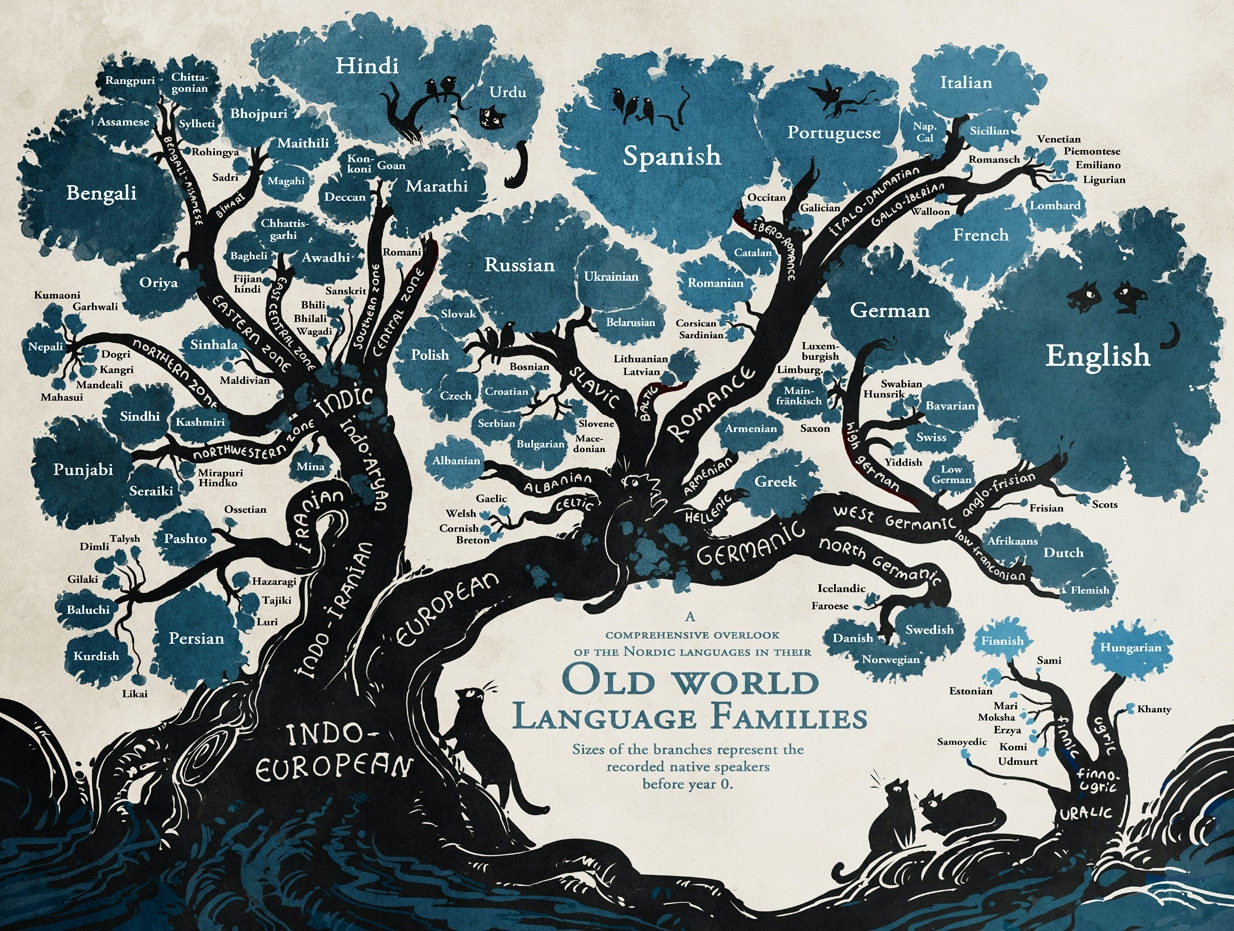
\includegraphics[width=0.75\textwidth]{history-trees/indo-european-1.jpeg}
\end{center}

\end{frame}

\begin{frame}
\frametitle{Some family trees}

\textbf{Sino-Tibetan} 

\begin{center}
    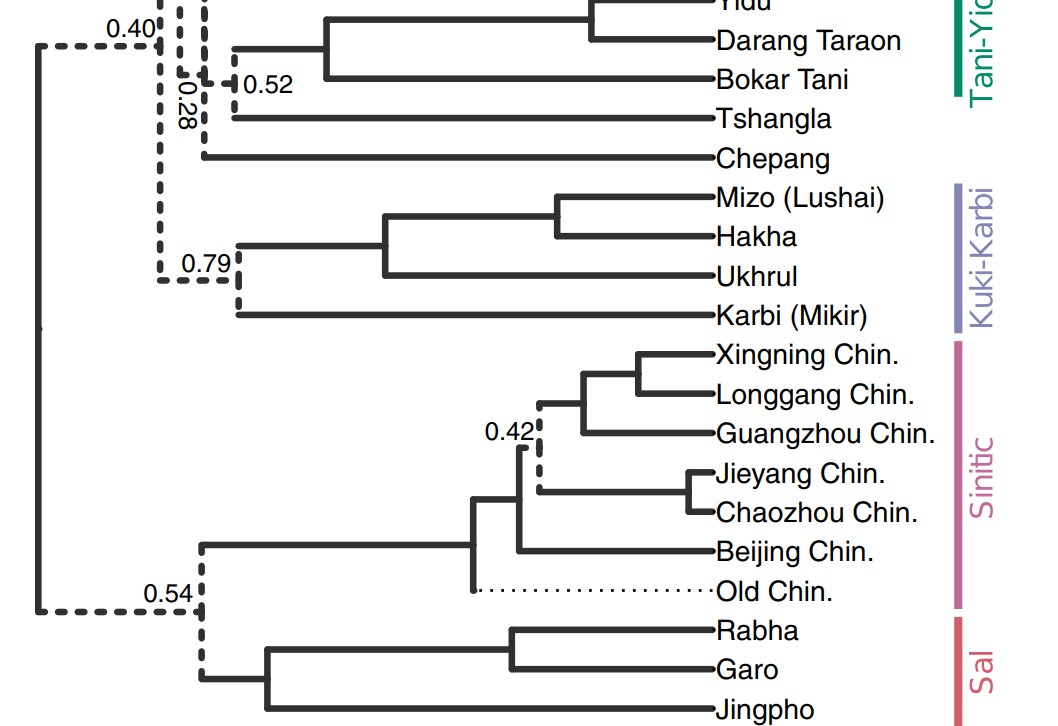
\includegraphics[width=0.6\textwidth]{history-trees/sino-tibetan-1.PNG}
\end{center}

\end{frame}

\begin{frame}
\frametitle{Conclusion}

\begin{itemize}
    \item Languages have their own way of historical development,
    quite similar to the case of microbes
    \item This fact can be used to build family trees of languages
    \item Linguists have already reconstructed several family trees for famous world languages
\end{itemize}    

\end{frame}

\end{document}